I am getting very, very tired of the abortion rights campaign from both
directions. This year has been a long, miserable year with tons of
horrible campaign ads about abortion. The pro-life campaigns have been
pushing to kick off sex panics of various sorts. Their rhetoric has been
more like what was seen right before the Rwandan genocides kicked off
than normal American political discourse, alas.

I am tired of existential, apocalyptic politics. I wound up writing this
letter and it was published in \emph{The} (Jefferson, Ohio)
\emph{Gazette} in the October 25th edition:

\begin{figure}
\centering
\pandocbounded{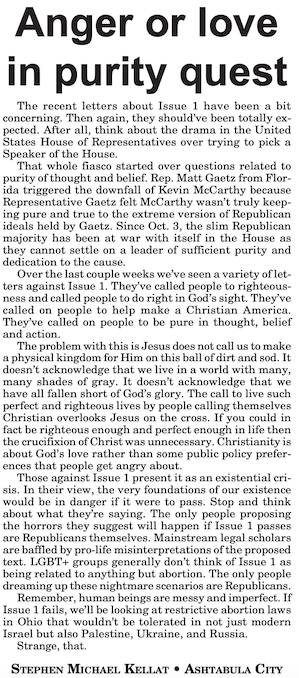
\includegraphics[keepaspectratio]{\%7B\%7Bsite.url\%7D\%7D/img/angerlove.jpg}}
\caption{Long letter to the editor in favor of the reproductive rights
amendment on the November 2023 general election ballot}
\end{figure}

I'm ready for this battle to end. The expectation that I have is that
Issue 1 will fail in Ashtabula County but pass statewide. I will be
quite shocked if it \emph{passes} in Ashtabula County. The key thing to
all of this is that if Issue 1 passes by an extremely large margin then
we have to reassess just how much Ohio falls on the MAGA/social
conservative spectrum.
